% !TEX root = ../swarthmore_talk.tex

% What is Arithmetic Geometry?
\begin{frame}[plain]
\ctext{What is Arithmetic Geometry?}
\end{frame}



% Arithmetic Geometry
\begin{frame}[plain] \frametitle{Arithmetic Geometry $\approx$ Diophantine Equations}
{\scriptsize Arithmetic Geometry is approximately the study of Diophantine equations. These are named after Diophantus of Alexandria (born $\approx$ A.D.~200), who wrote a thirteen volume set called the \textit{Arithmetica} of which six survive.}

\begin{dfn}[Diophantine Equation] \scriptsize
A Diophantine equation is a polynomial equation $f(x_1, x_2, \ldots, x_n)= 0$ with integer coefficients. One may consider the coefficients to come from other rings. 
\end{dfn}

\begin{minipage}{0.5\textwidth}
	\begin{figure}[ht]
	\centering
	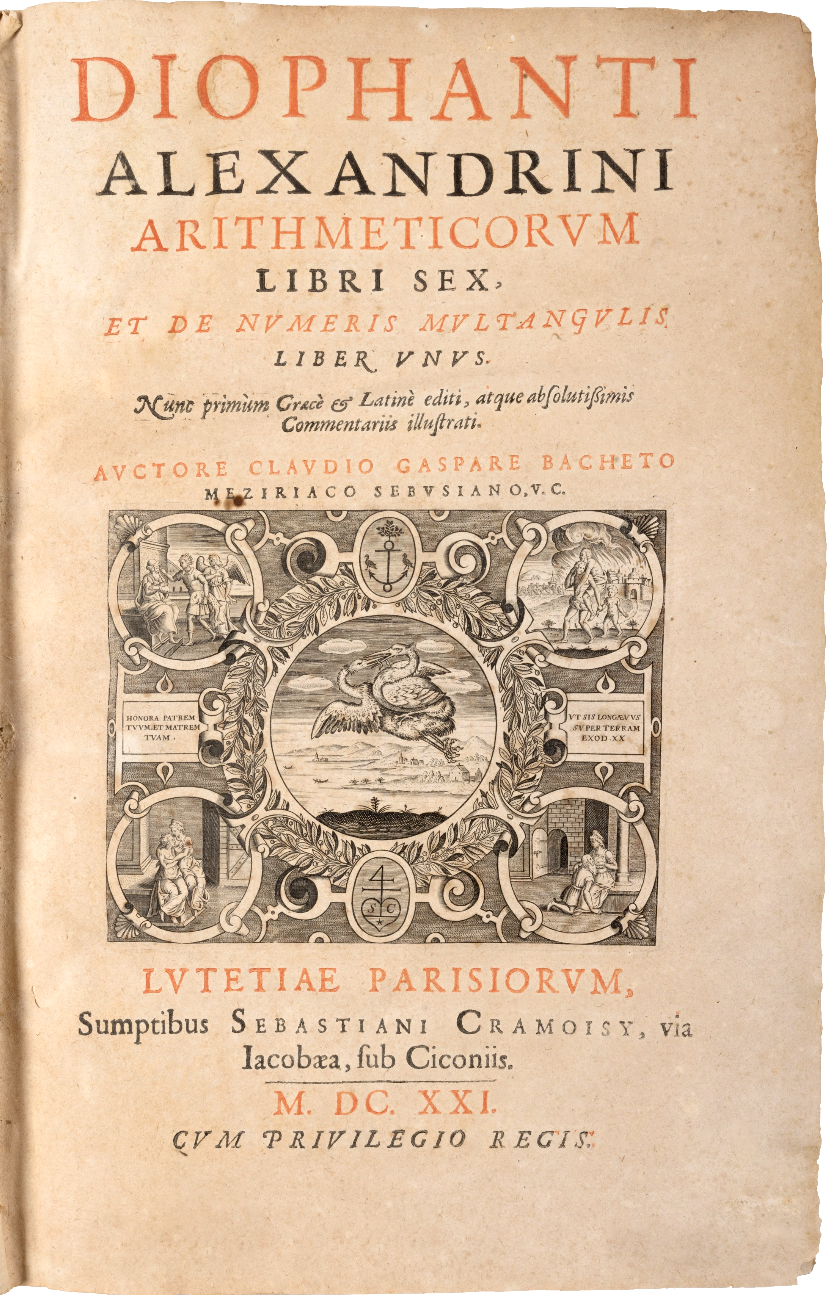
\includegraphics[width=0.6\textwidth]{images/diophantus.png}
	\end{figure}
\end{minipage}\begin{minipage}{0.55\textwidth} \scriptsize
We can ask number of questions:
	\begin{itemize}
	\item Can we determine if there are integer, rational, etc. solutions?
	\item If there are solutions, can we determine if there finitely or infinitely many?
	\item Can we find such solutions?
	\item Can we describe all the solutions?
	\item Is there an algorithm to do this generally?
	\end{itemize}
\end{minipage}
\end{frame}



% Polynomial Equations in One Variable
\begin{frame}[plain] \frametitle{Polynomial Equations in One Variable}
\small Consider the equation $f(x)= 0$, where $f(x)$ is a polynomial. \par\vspace{0.3cm}

{\itshape \bfseries Question:} Can we determine if there are `nice' solutions to a polynomial equation and, if so, determine what those solutions are? \par\vspace{0.3cm}

\begin{ex}
	\begin{itemize}
	\item $2x + 1= 5 \phantom{xxx..xx} \Longrightarrow \phantom{xxxx} x= 2$ \hfill 1 `nice' solution
	\item $x^2= 6 - x \phantom{xxx.xxx} \Longrightarrow \phantom{xxxx} x= -3, 2$ \hfill 2 `nice' solutions
	\item $x^2 - 2x - 4 = 0 \phantom{xx} \Longrightarrow \phantom{xxxx} x= 1 \pm \sqrt{5}$ \hfill 2 `not nice' solutions
	\item $x^2 + 1= 0 \phantom{xxx..xx} \Longrightarrow \phantom{xxxx.} x= \pm i$ \hfill No solutions?
	\end{itemize}
\end{ex} \par\vspace{0.3cm}
\end{frame}



% One Variable Polynomials
\begin{frame}[plain] \frametitle{The Case of One Variable Polynomials}
The case of one variable is finding the roots of a polynomial $f(x)= a_n x^n + a_{n-1} x^{n-1} + \cdots + a_0$.

\begin{thm}[Rational Roots Theorem]
Let $f(x)= a_n x^n + a_{n-1} x^{n-1} + \cdots + a_0$, where $a_i \in \Z$ and $a_0,a_n \neq 0$. Then the only rational solutions to $f(x)=0$ have $x= p/q$, where $p$ is an integer factor of $a_0$ and $q$ is an integer factor of $a_n$. 
\end{thm}

\begin{itemize}
\item We can determine if there are integer or rational solutions.
\item There are always at most $n$ solutions.
\item We can find all the integer or rational solutions.
\item The Rational Roots Theorem describes all the solutions.
\item The Rational Roots Theorem describes an algorithm to do this generally. 
\end{itemize}
\end{frame}



% Equations in Two Variables (Degree 1)
\begin{frame}[plain] \frametitle{Equations in Two Variables (Degree 1)}
What if we considered the equation $f(x, y)= 0$, where $f(x, y)$ is a polynomial of `degree 1' in two variables? \par\vspace{0.3cm}

{\itshape \bfseries Question:} Can we determine if there are `nice' solutions to a polynomial equation and, if so, determine what those solutions are? \par\vspace{0.3cm} 

\begin{ex}
	\begin{itemize}
	\item If $2x + 3y - 1= 0$, i.e. $2x+ 3y= 1$, there are infinitely many solutions. For example, $(x, y) = (-1, 1), (2, -1), (-4, 3), \ldots$. The solutions all have the form $(x, y)= (-1 - 3k, 1 + 2k)$, where $k$ is an integer. 
	\item If $2x - 4y - 5= 0$, i.e. $2x - 4y= 5$, there are no (integer solutions). However, there are rational solutions, e.g. $(\frac{5}{2}, 0)$ and $(0, -\frac{5}{4})$. In fact, all the solutions are rational (but not integer) and have the form $(k, \frac{4k + 5}{2})$, where $k$ is an integer. 
	\end{itemize}
\end{ex}
\end{frame}



% Two Variable Linear Equations
\begin{frame}[plain] \frametitle{Two Variable Linear Equations} \scriptsize
The case of two variable linear equations is finding integer (or rational) solutions to $ax + by= c$. This already involves a beautiful results from elementary number theory. Working modulo $n$ for some integer $n$ leads to the Chinese Remainder Theorem. 

\begin{thm}[Linear Diophantine Equations in Two Variables]
Let $a, b, c$ be integers with $a, b \neq 0$ and let $d= \gcd(a, b)$. The equation $ax + by= c$ has integer solutions if and only if $d \mid c$. If so, the equation has infinitely many solutions and all solutions have the form\dots
	\[
	x= x_0 + \frac{b}{d} \, k, \quad y= y_0 - \frac{a}{d} \, k,
	\]
where $(x_0, y_0)$ is a solution and $k$ is an integer. 
\end{thm}

\begin{itemize}
\item We can determine if and when there are integer solutions.
\item If there are integer solutions, there are infinitely many and we can parametrize them.
\item There are always infinitely many rational solutions and we can parametrize the solutions.
\item There is an algorithm in both the integer and rational case. 
\end{itemize}
\end{frame}



% What about higher degree equations?
\begin{frame}[plain]
\ctext{What about higher degree equations?}
\end{frame}



% Higher Degree Equations
\begin{frame}[plain] \frametitle{Higher Degree Equations}

What about equations in two variables with higher degree? \vspace{0.3cm}

\begin{ex}
	\begin{itemize}
	\item The equation $y^2 + 108= x^3$ has no solutions. \vspace{0.3cm}
	\item The equation $y^2= x^3 - 2$ only has the solutions $(x, y)= (3, \pm 5)$. \vspace{0.3cm}
	\item The equation $x^2 + y^2= 4$ has infinitely many solutions. \vspace{0.3cm}
	\item The equation $x^2 - 1141y^2= 1$ has solutions but the `simplest' solution, i.e. `first' integer solution, is\dots
		\[
		\begin{aligned}
		x&= 1036782394157223963237125215 \\
		y&= 30693385322765657197397208
		\end{aligned}
		\]
	\end{itemize}
\end{ex}
\end{frame}



% Quadratic Diophantine Equations --- Conics
\begin{frame}[plain] \frametitle{Quadratic Diophantine Equations --- Conics} \small
The case of two variable, quadratic Diophantine equations is the study of `nice' points on various conic sections, i.e. the set of zeros for a polynomial $F(x,y)= ax^2+bxy + cy^2 + ex+fy+h \in \Q[x,y]$. \pspace
	
	\begin{figure}[ht]
	\centering
	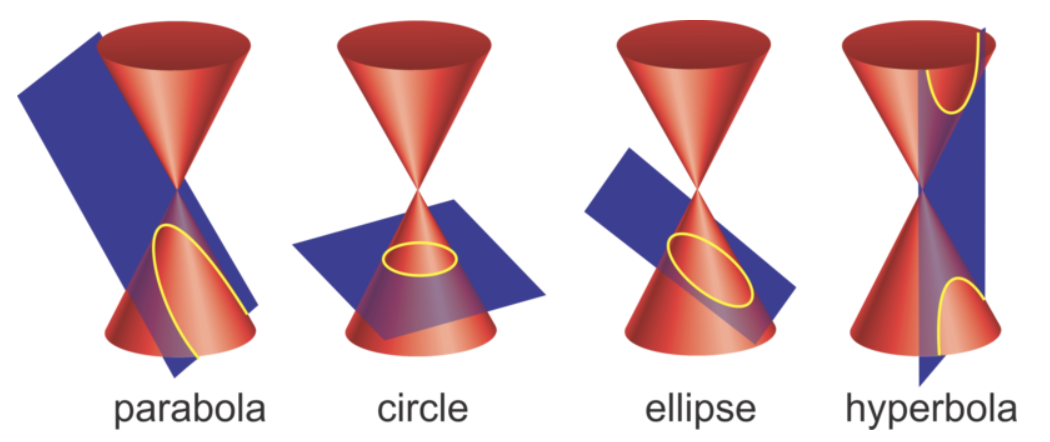
\includegraphics[width=0.65\textwidth]{images/conics.png}
	\end{figure}

\begin{itemize}
\item The set of real solutions to these polynomials are circles, ellipses, parabolas, hyperbolas, and degenerate cases like a point or pair of lines. Therefore, we seek `nice' points on these surfaces.

\item We want our curves to be smooth, i.e. there is no solution (over $\C^2$) to
	\[
	F(x,y)= \dfrac{\partial F}{\partial x}(x,y)= \dfrac{\partial F}{\partial y}(x,y)= 0
	\]
\end{itemize}

\end{frame}



% Examples
\begin{frame}[plain,t]
\frametitle{\textcolor{white}{Finding Rational Points on Conics}}
	\[
	x^2 + y^2 = 1 
	\] \vfill
	\[
	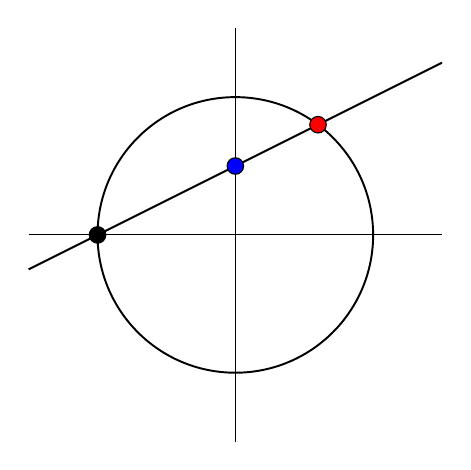
\begin{tikzpicture}[scale=1.75]
	\draw (-1.5,0) -- (1.5,0);
	\draw (0,-1.5) -- (0,1.5);

	\draw[line width=0.7] (-1.5,-0.25) -- (1.5,1.25);
	\draw[line width=0.7] (0,0) circle (1);
	
	\draw[fill=black] (-1,0) circle (0.06);
	\draw[fill=blue] (0,0.5) circle (0.06);
	\draw[fill=red] (0.6,0.8) circle (0.06);
	\end{tikzpicture}
	\] \vfill
	\[
	C(\Q)= \{ (-1,0) \} \cup \left\{ \left(\dfrac{1-t^2}{1+t^2}, \dfrac{2t}{1+t^2} \right) \colon t \in \Q \right\}
	\] \pspace
\end{frame}



% Local-to-Global
\begin{frame}[plain] \frametitle{Local-Global Principles}
The `projection' method does not always work---we need a rational point at the start. For example, the following circle has no rational point:
	\[
	x^2 + y^2= 3
	\]
Transforming this into an integer equation, one can work modulo 4 and show there is no solution, which implies there is no rational solution. In fact, all conics that do not have a rational point fail some type of congruence condition. 

\begin{prin}[Hasse, Local-Global Principle]
A collection of equations has a solution `if and only if' it has a solution in $\R$ and $\Q_p$ for all $p$.
\end{prin} 
\end{frame}



% Falting's Theorem
\begin{frame}[plain] \frametitle{The Case of Higher Degree Equations} \small

\begin{thm}[Mordell, 1922, Faltings, 1983]
If $\mathcal{C}$ is a curve over $\Q$ of genus $g$ at least 2, then $\mathcal{C}$ has at most finitely many rational points. 
\end{thm}

	\begin{figure}[ht]
	\centering
	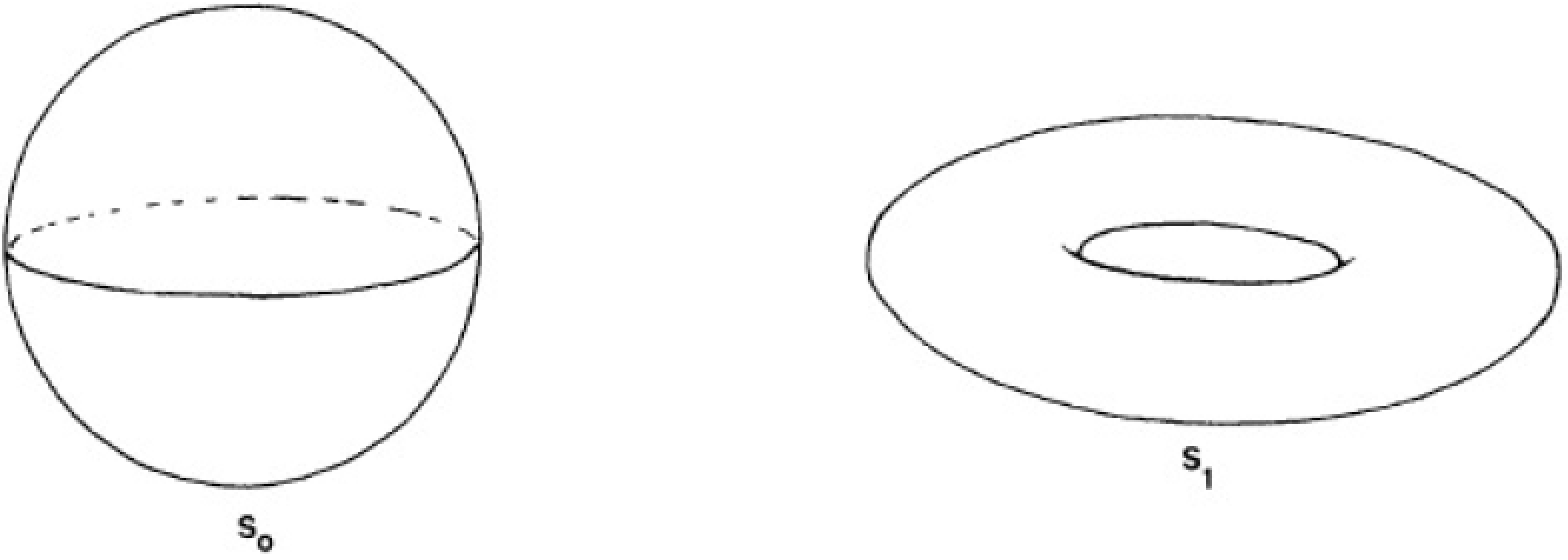
\includegraphics[width=0.35\textwidth]{images/genus1.png} \quad
	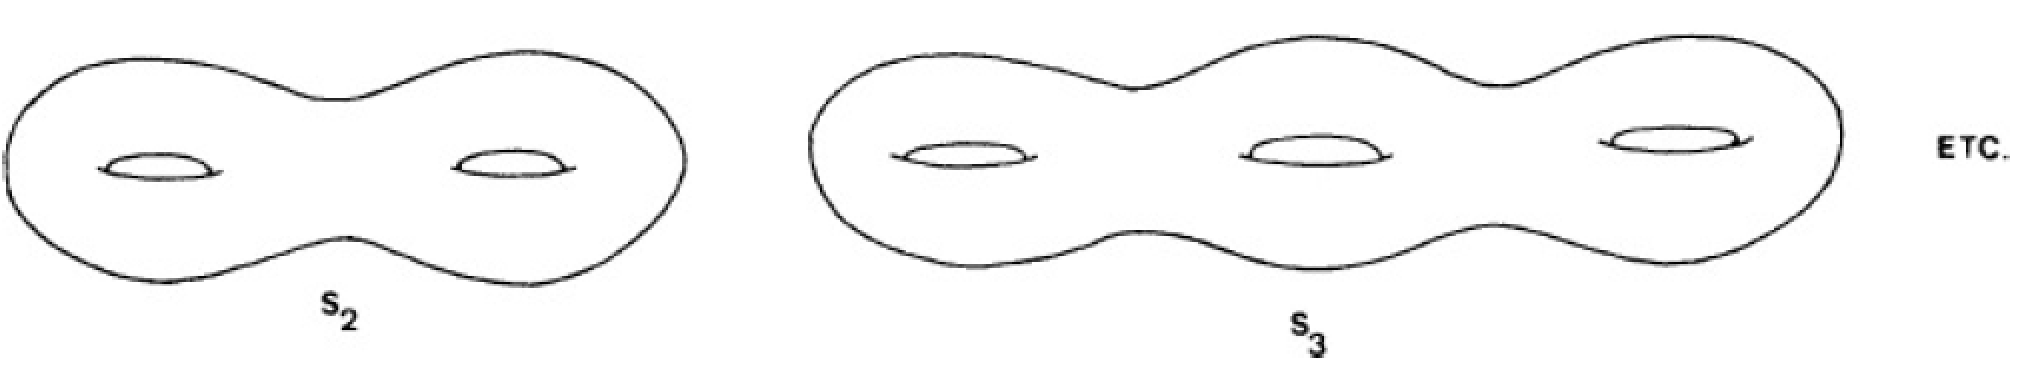
\includegraphics[width=0.45\textwidth]{images/genus2.png}
	\end{figure}

\begin{rem}
If $\mathcal{C}$ is a nonsingular, projective plane curve of degree $d$ is given by\dots
	\[
	g= \dfrac{(d - 1)(d - 2)}{2}
	\]
For a non-singular hypersurface $H$ of degree $d$ in $\mathbb{P}^n$, we have $g= \binom{d - 1}{n}$. Topologically, the genus is the number of `holes.' 
\end{rem}
\end{frame}



% Isosceles Triangle Problem
\begin{frame} \frametitle{Isosceles Triangle Problem} \footnotesize
{\itshape Does there exist a rational right triangle and a rational isosceles triangle that have the same area and the same perimeter?} \pspace

If yes, we can find $t, u \in \Q$, $0 < t < 1$, $0 < u < 1$, and $k > 0$. 
	
	\begin{figure}[!ht]
	\centering
	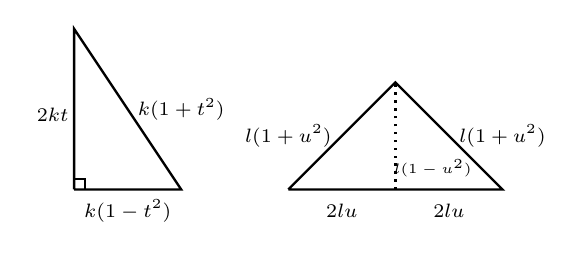
\begin{tikzpicture}[scale=0.68]
	\draw[line width=0.03cm] (0,0) -- (0,3) -- (2,0) -- (0,0);
	\draw[line width=0.03cm] (0,0.2) -- (0.2,0.2) -- (0.2,0);
	\node at (1,-0.4) {\scriptsize$k(1-t^2)$};
	\node at (-0.4,1.4) {\scriptsize$2kt$};
	\node at (2.0,1.5) {\scriptsize$k(1+t^2)$};
	
	\draw[line width=0.03cm] (4,0) -- (6,2) -- (8,0) -- (4,0);
	\draw[line width=0.03cm,dotted] (6,0) -- (6,2);
	%\draw[line width=0.03cm] (5.85858,1.85858) -- (6,1.71716) -- (6.14142,1.85858);
	\node at (4,1) {\scriptsize$l(1+u^2)$};
	\node at (8,1) {\scriptsize$l(1+u^2)$};
	\node at (5,-0.4) {\scriptsize$2lu$};
	\node at (7,-0.4) {\scriptsize$2lu$};
	\node at (6.7,0.4) {\tiny$l(1-u^2)$};
	\end{tikzpicture}
	\end{figure} 
With even more algebra, this is the same as finding a rational solution $(x,y)$ to 
	\[
	y^2= x^6 + 12x^5 - 32x^4 + 52x^2 - 48x + 16
	\]

\begin{thm}[Hirakawa, Matsumura 2018]
Up to similitude, there exists a unique pair of rational right triangles and a rational isosceles triangle which have the same perimeter and the same area. The unique pair consists of the right triangle with side $(377,135,352)$. and isosceles triangle with sides $(366,366,132)$. 
\end{thm}
\end{frame}



% Sweet Spot
\begin{frame}[plain]
\ctext{This leaves the `sweet spot' of cubic equations}
\end{frame}



% Elliptic Curves
\begin{frame}[plain]
\ctext{Elliptic Curves}
\end{frame}



% Quote
{\setbeamertemplate{background canvas}{
\tikz[remember picture,overlay]
	\node[opacity=0.3] at (current page.center) {
	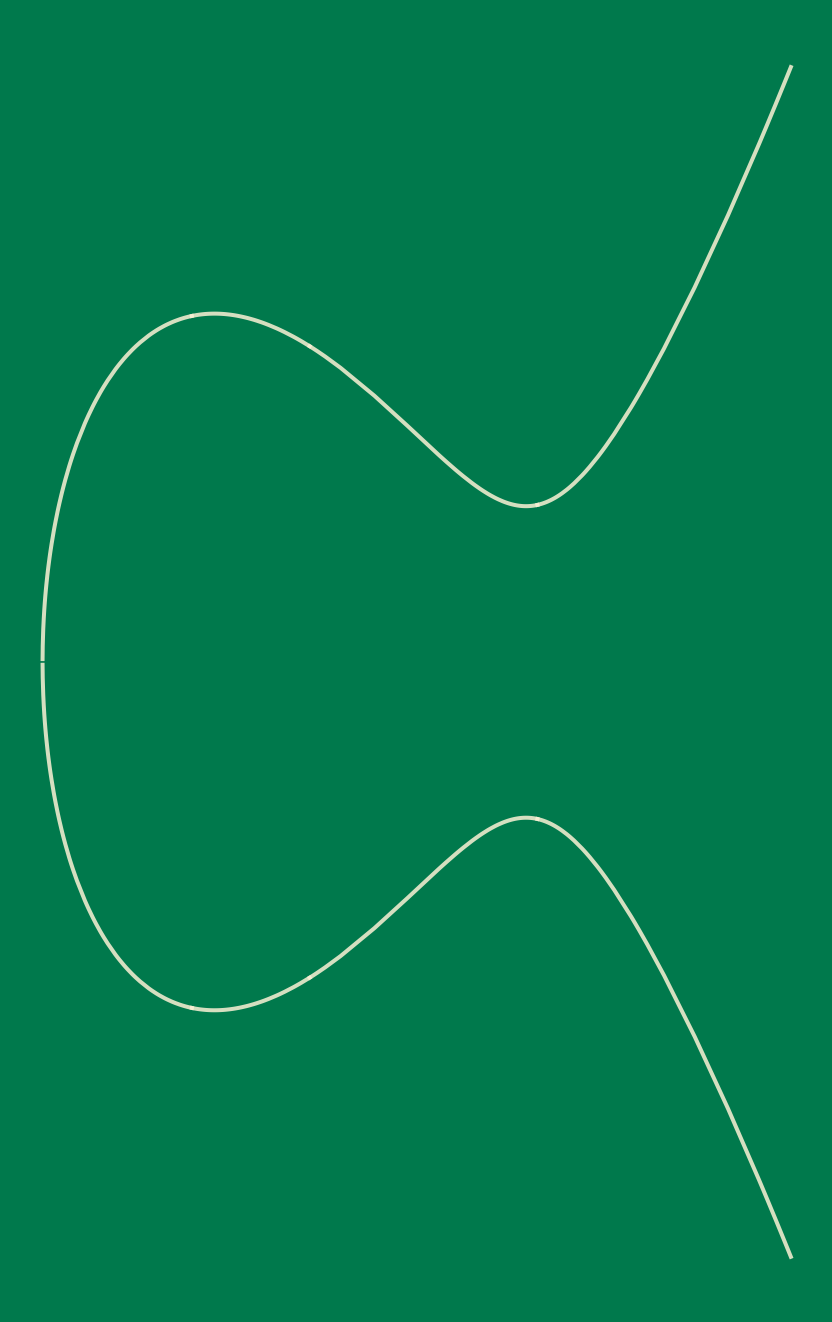
\includegraphics[width=1.25\paperwidth,
	height=1.25\paperheight]{images/curve2.png}};} 
\begin{frame}[plain]
	\begin{minipage}{0.18\textwidth}
 	\begin{figure}[h]
	\centering
	\fbox{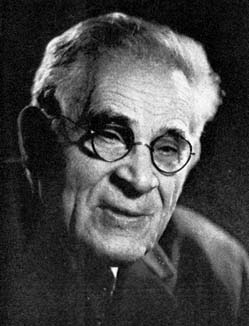
\includegraphics[width=1.1\textwidth]{images/mordell.jpg}} \par
	{\small 1888 -- 1972}
	\end{figure}
	\end{minipage} \hspace{0.2cm} \begin{minipage}{0.76\textwidth}
	\begin{center} \phantom{.} \par \phantom{.} \par
	{\itshape ``Mathematicians have been familiar with very few questions for so long a period with so little accomplished in the way of general results, as that of finding the rational [points on elliptic curves].''} \\
	 \phantom{x}\hfill-- L.J. Mordell, 1922
	\end{center}
 	\end{minipage}
\end{frame}
}